\documentclass[border=4pt]{standalone}
\usepackage{tikz}
\usetikzlibrary{positioning, arrows.meta, shapes.geometric, calc, fit, backgrounds}
\usepackage{amsmath,amssymb}
\begin{document}
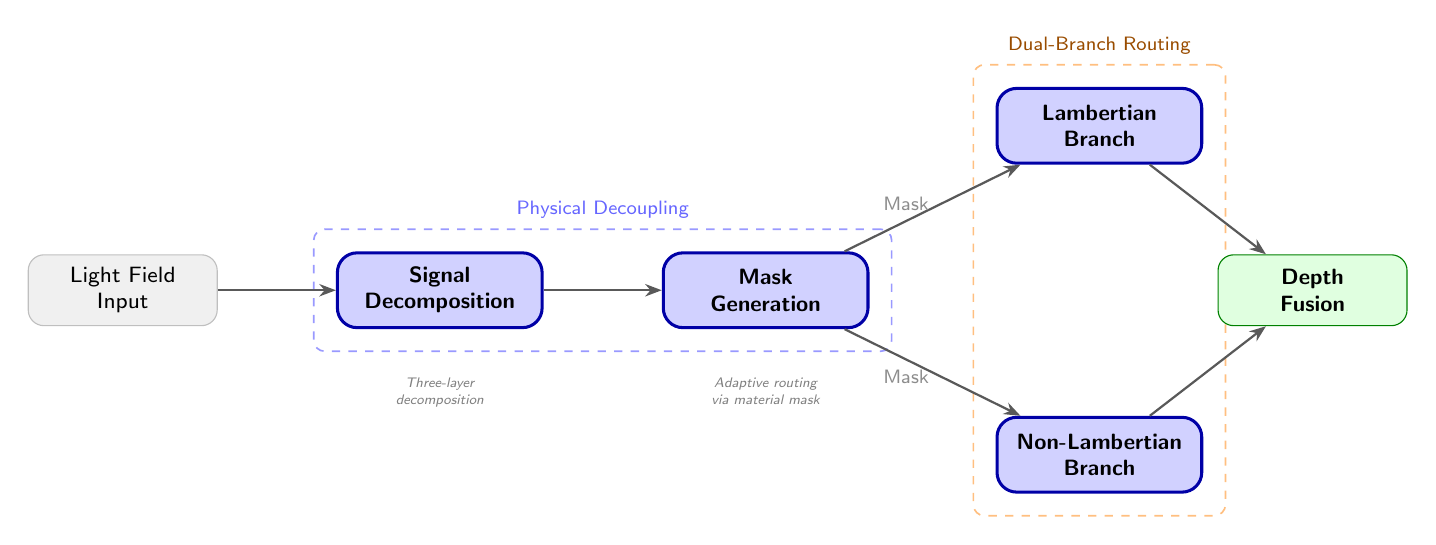
\begin{tikzpicture}[
  input/.style={draw, rounded corners=2mm, minimum width=2.4cm, minimum height=0.9cm,
                fill=gray!12, draw=gray!50, align=center, font=\sffamily\footnotesize},
  innov/.style={draw, rounded corners=2.5mm, minimum width=2.6cm, minimum height=0.95cm,
                fill=blue!18, draw=blue!65!black, line width=1.1pt, align=center,
                font=\sffamily\footnotesize\bfseries},
  output/.style={draw, rounded corners=2mm, minimum width=2.4cm, minimum height=0.9cm,
                 fill=green!12, draw=green!50!black, align=center,
                 font=\sffamily\footnotesize\bfseries},
  arr/.style={-{Stealth[length=6pt]}, thick, color=black!65},
  lbl/.style={font=\sffamily\scriptsize, text=black!45},
  gbox/.style={draw=#1, dashed, rounded corners=4pt, inner sep=8pt, line width=0.6pt},
  annot/.style={font=\sffamily\tiny\itshape, text=black!50, align=center},
]

% === Nodes ===
\node[input] (m1) {Light Field\\Input};

\node[innov, right=1.5cm of m1] (m2) {Signal\\Decomposition};

\node[innov, right=1.5cm of m2] (m3) {Mask\\Generation};

\node[innov, above right=1.1cm and 1.6cm of m3] (m4) {Lambertian\\Branch};

\node[innov, below right=1.1cm and 1.6cm of m3] (m5) {Non-Lambertian\\Branch};

\path (m4) -- (m5) coordinate[midway] (midBranch);
\node[output, right=1.5cm of midBranch] (m6) {Depth\\Fusion};

% === Arrows ===
\draw[arr] (m1) -- (m2);
\draw[arr] (m2) -- (m3);
\draw[arr] (m3) -- node[lbl, above, pos=0.35] {Mask} (m4);
\draw[arr] (m3) -- node[lbl, below, pos=0.35] {Mask} (m5);
\draw[arr] (m4) -- (m6);
\draw[arr] (m5) -- (m6);

% === Grouping (background layer) ===
\begin{scope}[on background layer]
  \node[gbox=blue!40, fit=(m2)(m3),
        label={[lbl, text=blue!60]above:Physical Decoupling}] {};
  \node[gbox=orange!50, fit=(m4)(m5),
        label={[lbl, text=orange!60!black]above:Dual-Branch Routing}] {};
\end{scope}

% === Annotations ===
\node[annot, below=0.5cm of m2] {Three-layer\\decomposition};
\node[annot, below=0.5cm of m3] {Adaptive routing\\via material mask};

\end{tikzpicture}
\end{document}